\documentclass[10pt,onecolumn,twoside,letterpaper]{article}
\usepackage[text={7.7in,9.5in},centering]{geometry}
\usepackage[utf8]{inputenc}
\usepackage[spanish,es-nodecimaldot]{babel}

\usepackage{hyperref}

\usepackage{multicol}
\usepackage{wrapfig}

\usepackage{amsmath,amssymb,amsthm}

\usepackage{harvard}% bibliographystyle: apsr, agsm, dcu, kluwer, nederlands
\newcommand{\myreferences}{../../bib/library}
\usepackage{graphicx}
\graphicspath{{../../images/}}
\usepackage{amssymb}
\usepackage{fancyhdr}
\usepackage{color}
\usepackage{colortbl}
\definecolor{gray}{cmyk}{0.0,0.0,0.0,0.60}

\usepackage{float}

%\usepackage{auto-pst-pdf}
%\usepackage{pst-all}

\usepackage{mcode}
%\usepackage[numbered]{mcode}
%\usepackage{lipsum}

\pagestyle{fancy}
\fancyhf{}
\fancyhead[RO]{\small{\textcolor{gray}{\textsc{Hacia un framework de locomoci\'on b\'ipeda, evolutiva y flexible}}}}
\fancyhead[LO]{
\includegraphics[scale=0.05]{unlogo.png}}
\fancyhead[LE]{
\includegraphics[scale=0.05]{unlogo.png}\quad\small{\textcolor{gray}{\textsc{Control Inteligente 2015-01}}}}
\fancyhead[RE]{\small{\textcolor{gray}{\textsc{TALLER 03}}}}
\fancyfoot[CO,CE]{\thepage}
\fancyfoot[LO,RE]{\scriptsize{\textcolor{gray}{\emph{Version 0.1}}}}

\title{\vspace{-0.8cm}
\includegraphics[scale=0.12]{unescudobn.png}\\\vspace{-0.0cm}
  \LARGE \textbf{Taller 3 - Sistemas, Modelos Difusos y T\'ecnicas de Construcci\'on}}
\author{J.A. Castillo-Le\'on\thanks{jacastillol@unal.edu.co} \and Ronny Gelleschus\thanks{rgelleschus@unal.edu.co}}
\date{}

\begin{document}
\maketitle
\begin{abstract}\noindent\small\textit{(poner el abstract aca bla, bla blah) En el siguiente documento se hacen ejercicios de repaso de los fundamentos b\'asicos de los conjutos difusos y las relaciones difusas. La implicaci\'on es la relaci\'on que mas se detalla. Finalmente un sistema experto de toma de decisiones se construye y analiza con MATLAB.}
\end{abstract}\vspace{1cm}

%\begin{multicols}{2}

\par{\bf \large Punto 1:} Diagrama de bloques gen\'erico para un sistema difuso basado en reglas. Nombre y funci\'on de sus diferentes componentes.\\
\begin{figure}[!htb]
  \centering
  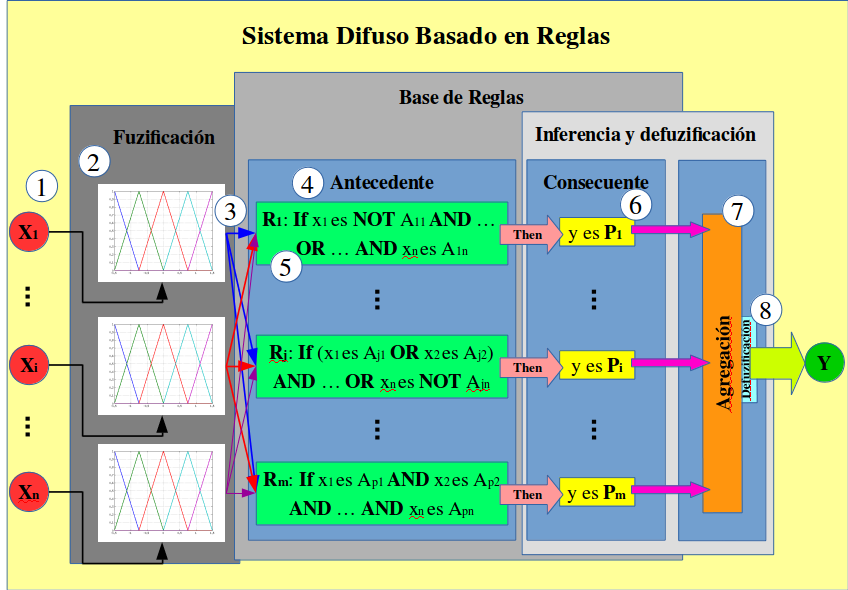
\includegraphics[width=0.85\textwidth]{Rule-BasedFuzzySystem02.png}
  \caption{Diagrama general de sistema difuso basado en reglas}
  \label{fig:ruleBasedSystem}
\end{figure}

En la Figura \ref{fig:ruleBasedSystem}., se describe los componentes g\'enericos de un sistema MISO. Comenzando por \raisebox{.5pt}{\textcircled{\raisebox{-.9pt} {1}}}, la entrada al sistema difuso es un vector $\mathbf{X}\,=\,\left[x_1,x_2,\ldots,x_i,\ldots,x_n\right]\in\mathcal{D}\subset\mathbb{R}^n$, dicho vector forma las \emph{variables base} del concepto de un conjuto de \emph{variables ling\"uisticas}. Esta entrada vectorial es analizada componente por componente \raisebox{.5pt}{\textcircled{\raisebox{-.9pt} {2}}}, por el proceso llamado \emph{fuzificaci\'on}, en el cual se obtienen los valores de las \emph{funciones de pertenencia} que representan a las \emph{etiquetas ling\"uisticas} de cada variable ling\"uistica.\\
\par En \raisebox{.5pt}{\textcircled{\raisebox{-.9pt} {3}}}, la salida del fuzificador entrega los valores de pertenencia $\mu_{A_{ij}}(x_i)$ de cada una de las variables $x_i$ a sus respectivas reglas $\mathcal{R}_k$ de la base del conocimiento para que puedan ser evaluadas. Esta base de reglas es editada usando reglas \textbf{if-then}. Los antecedentes \raisebox{.5pt}{\textcircled{\raisebox{-.9pt} {4}}} son proposiciones que utilizan operadores de conexi\'on \textbf{AND} y \textbf{OR} adem\'as de la operaci\'on de complemento \textbf{NOT} (como es el caso del modelo relacional), auque generalmente solo se usa la \textbf{AND} (este es el caso de los modelos de Mamdani, Singleton y T-S). \raisebox{.5pt}{\textcircled{\raisebox{-.9pt} {5}}} Al momento de la implementaci\'on se usa \emph{t}-norma para la conjunci\'on y la \emph{t}-conorma para la disyunci\'on. El n\'umero de reglas que salen de un sistema con $n$ entradas y $p$ etiquetas ling\"uisticas para entrada, se tiene un m\'aximo de reglas-\textbf{AND}, $m\,=\,n^p$.\\
\par \raisebox{.5pt}{\textcircled{\raisebox{-.9pt} {6}}} El consecuente depende del modelo puede ser una proposici\'on que implica un conjuto difuso con en el caso Mamdani o una funci\'on concreta con en el caso T-S. En el caso T-S en la \emph{implicaci\'on}, \raisebox{.5pt}{\textcircled{\raisebox{-.9pt} {7}}} a la final todas las reglas se deben tener en cuenta para hacer una ponderaci\'on de salida, en este se hace una suma ponderada de los valores de cumplimiento (\emph{degree of fulfillment}). \emph{Defuzificaci\'on} \raisebox{.5pt}{\textcircled{\raisebox{-.9pt} {8}}} Cunado la salida es difusa se requiere un paso adicional de defuzificaci\'on, como en el caso Mamdani, que utiliza metodos de COG y MOM.

%Aquí utilizaría algo como en la presentación del profe (capítulo 3), página 14 en el documento que nos envió. Sin embargo para mí eso no es un diagrama de bloques, se tiene que cambiar los señales (y evitar el uso de un "BUS" de señales) y los símbolos de los elementos del sistema a bloques simples. No sé con cuál programa podemos hacerlo. Tú tienes una idea?\\
\par{\bf \large Punto 2:} Algorithmo Mamdani (\cite{Babuska1999}, página 37)\\
Primero se tiene que calcular el grado de cumplimiento del conjunto en la entrada para cada regla. La fórmula general es $\beta_i = \max(\min(\mu_{A'}(x),\mu_{A_i}(x)))$. En el caso de una entrada concreta $x_0$ eso se simplifica a $\beta_i=\mu_{A_i}(x_0)$.\\
En el segundo paso se calcula el conjunto que resulta para cada regla: $\mu_{B'_i}(y)=\beta_i\cdot \mu_{B_i}(y)$.\\
Al final se agrega el resultado calculándo el máximo de todos los $\mu_{B'_i}$ en cada punto $y\in Y$: $\mu_{B'}(y)=\max(\mu_{B'_i}(y))$.\\
Para una entrada $x_0=2$ y con las reglas establecidas en la tarea eso significa:
\begin{enumerate}
\item $\beta_1=0.6$ y $\beta_2=0.4$.
\item $B'_1=[ 0.6/4; 0.6/5; 0.18/6]$ y $B'_2=[0.04/4; 0.36/5; 0.4/6]$.
\item $B'=[0.6/4; 0.6/5; 0.4/6]$.
\end{enumerate}

\par{\bf \large Punto 3:} Modelo Takagi-Sugeno\\
$z = \frac{\sum_{i=1}^{K}\beta_i\cdot z_i(x,y)}{\sum_{i=1}^{K} \beta_i}$, donde $\beta_i$ es el grado de cumplimiento de una regla y $K$ el número de reglas. Para calcular el grado de cumplimiento de cada regla $i$ se utilizó $\beta_i=\min(\mu_{A_i}(x),\mu_{B_i}(y))$. Entonces $z= \frac{0.1\cdot 6+0.9\cdot 7+0.1\cdot 14+0.1\cdot 7}{0.1+0.9+0.1+0.1}=7.5$.\\

\par{\bf \large Punto 4:} Construcción de un modelo difuso basado en conocimiento (\cite{Babuska1999}, página 79)
\begin{enumerate}
\item Selección de los variables de entrada y salida, la estructura de las reglas y los métodos de inferencia y defusificación
\item Decisión cuántos términos linguísticos se tendrá en el sistema y definición de las funciones de membrencia correspondientes
\item Formulación del conocimiento en forma de reglas If-Then
\item Validación del modelo (normalmente usando valores reales disponibles). Si el modelo no cumple con las espectativas, entonces iteración de los pasos anteriores.
\end{enumerate}

\par{\bf \large Punto 5:} Sistema dinámico modelado con singleton: $y(k+1)\,=\,f(y(k),u(k))$\\
\par{\bf 5.1: Ejemplo de modelo aproximado con singleton}
\par Tomando el ejemplo 5.1 de \cite{Babuska1999} que utiliza un modelo T-S para aproximar sistema discreto $y(k+1)\,=\,y(k)+u(k)e^{-3\left|y(k)\right|}$ utiliza reglas de la forma:\\
$R^{i}$: \textbf{If} $y(k)$ is $A_{i}$ \textbf{then} $y(k+1)=a_iy(k)+b_iu(k)$.
\par Los p\'arametros $\left\{a_i,b_i\right\}$ son ajustados por \emph{m\'inimos cuadrados}. La ecuaci\'on 5.2 de \cite{Babuska1999} fue utilizada para comprobar el ejemplo de dichas notas. Se destaca que $\mathbf{X}_e$ se utiliz\'o sin el uso del vector unario (ver Figura \ref{fig:AproxTS}). Se utiliz\'o siete funciones de pertenecia para la \'unica variable de entrada
\begin{figure}[!htb]
  \centering
  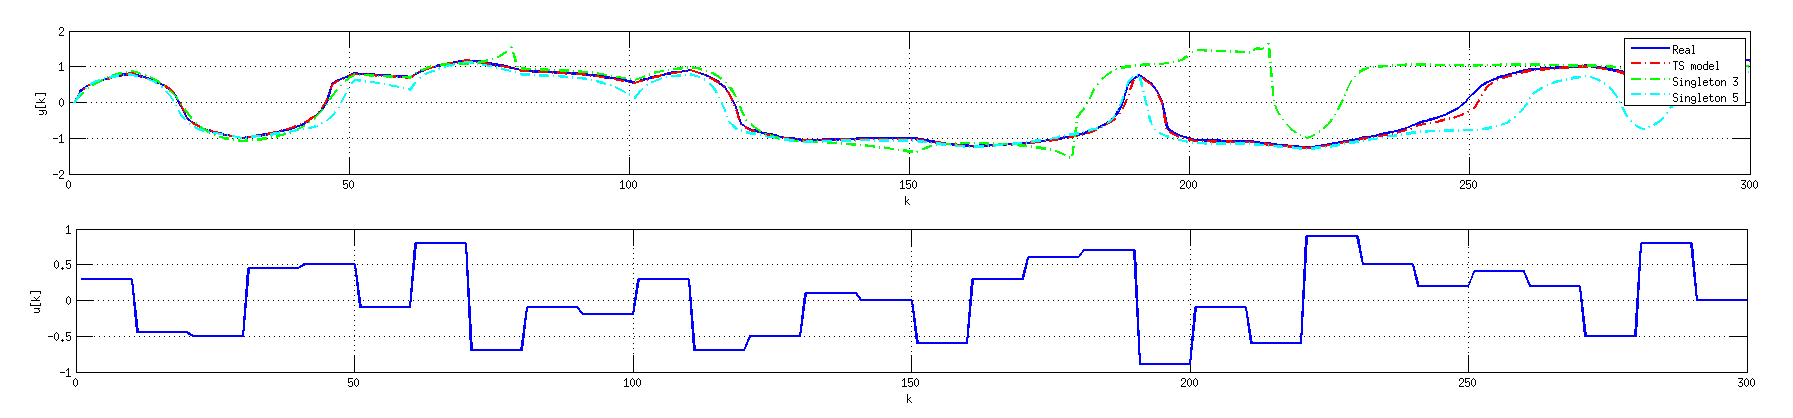
\includegraphics[width=0.9\textwidth]{ApproxTS5-1.png}
  \caption{Aproximaci\'on usando TS}
  \label{fig:AproxTS}
\end{figure}

\par Para aproximar usando singleton, las reglas tomar\'ian la siguiente forma:\\
$R^{i}$: \textbf{If} $y(k)$ is $A_{i}$ \textbf{and} $u(k)$ is $B_{j}$ \textbf{then} $y(k+1)=c_k$.\\
\par Si se toman 3 funciones de pertenencia por entrada se tendrian 9 reglas. Se resuelven los parametros con m\'inimos cuadrados nuevamente, la ecuaci\'on 5.2 de \cite{Babuska1999} es tomada esta bvez con $\mathbf{X}_e\,=\,\mathbf{1}$ como el vector unario, para resolver unicamente los parametros del singleton (ver Figura \ref{fig:AproxTS}). La soluci\'on es bastante diferente comparada con la TS, sin embargo al subir de 3 a 5 funciones de pertenencia, la solucion es mas acertada pero sigue siendo inferior a la TS.\\
\par{\bf 5.2: Parametros para afinar}
\par Los coeficientes $c_i$ son los valores a encontrar y son hallados por m\'inimos cuadrados. Para las nueve reglas los singleton son: $c=[-1.1717,-0.9257, 1.9182,-1.5349, 0.0566, 1.4627,-1.6685, 0.6578, 1.2637]^T$, las funciones de pertenencias son triangulares y se distribuyen equidistantes en el rango de las variables. Para mejorar la soluci\'on se puede modificar los parametros de las funciones de pertenencia, pero esta b\'usqueda debe ser planteada como un problema de optimizaci\'on y se usa generalmente algorimos evolutivos. 

\par{\bf \large Punto 6:} Ecuaci\'on general modelo dinamico tipo NARX para SISO\\
%No estoy seguro si también se tiene que incluir el $n_d$ en los términos de $y$, pero me imagino que sí porque se los usa para la parte autoregresiva (depende de si el elemento con el tiempo muerto está en el sistema o sólo en la medición del set point que tal vez viene de otro sistema?):\\ 
$y(k+1)=f_{NL}(y(k-n_d),y(k-n_d-1),\dots,y(k-n_d-n_y+1),u(k-n_d),u(k-n_d-1),\dots,u(k-n_d-n_u+1))$\\
$y$: valores de la salida (anteriores y futuro)\\
$u$: valores de la entrada anteriores\\
$k$: instante de tiempo actual\\
$n_y$, $n_u$: número de instantes anteriores que se tiene en cuenta para calcular $y(k+1)$\\
$n_d$: número de instantes anteriores que no se puede utilizar por el tiempo muerto\\
$f_{NL}$: función (en general no lineal) que relaciona $y(k+1)$ con los valores anteriores de $y$ y $u$\\
Un ejemplo reportado en la literatura es \cite{Ho2008}

\par{\bf \large Punto 7:} Modelo Semi-mechan\'istico\\
\par(\cite{Babuska1999}, página 89) Un modelo semi-mecanístico es un modelo que combina partes \emph{caja blanca} y \emph{caja negra}. Así se puede evitar que se utiliza métodos de aproximación y identificación en relaciones físicos que se conoce exactamente.
\par{\bf 7.1: Selecci\'on de estructura y estimaci\'on par\'ametros}\\
\par En general en la selección de estructura para un sistema difuso se tiene que tener en cuenta la selección de variables de entrada y salida, la estructura de las reglas, el número y el tipo de funciones de pertenencia para cada variable y los mecanismos de inferencia, de conección (definición de AND o OR) y la defuzzyfication. En el modelado semi-mecanístico se sabe unos mecanismos del sistema real, para las cuáles no se necesita un modelo difuso. Entonces se tiene que asignar cuáles variables de entrada van a ser procesadas en el modelo difuso y cuáles en un modelo clásico. Para estas partes del sistema la estimación de parámetros podría ser necesario para unas constantes, pero no para todo el sistema.
\par Volviendo al ejemplo del punto 5 de esta tarea, el hecho de conocer la ecuaci\'on discreta del sistema $y(k+1)\,=\,y(k)+u(k)e^{-3\left|y(k)\right|}$ nos permite seleccionar una estructura de reglas mas apropiada que solo depende de $y(k)$, ya que la no linealidad del problema solo depende de $y(k)$ y modificar los minimos cuadraros para la estimaci\'on de los par\'ametros a solo siete parametros obteniendo una mejor aproximaci\'on con solo siete reglas. Mientras que al considerar dos entradas $y(k)$ y $u(k)$ se requiere de 9 reglas para singleton-3 y 25 reglas para singleton-5 (Figura \ref{fig:AproxTS}.) con un desempeño pobre.
\par{\bf 7.2: Diferentes aspectos para tener en cuenta en la selecci\'on de la estructura}\\
\par En el modelado semi-mecanístico de modelos difusos se tiene que tener en cuenta varias preguntas:
\begin{itemize}
\item Cuáles partes del sistema se puede modelar por ecuaciones diferenciales basadas en leyes naturales como un balance de masa o de energía?
\item Qué modelo para estas partes sería computacionalmente menos difícil, la ecuación diferencial o un modelo difuso?
\item Qué tan grande sería la diferencia entre los resultados utilizando un modelo basado en leyes naturales y un modelo difuso?
\end{itemize}
\par Algunas conclusiones del punto cinco. Primero: si se conoce $n_y$, $n_u$ y $n_d$, se puede reducir el numero de reglas. Segundo en las consecuencias se puede reducir el n\'umero de parametros, basta con mirar las no linealidades y su dependencias con $y$'s y $u$'s observar que los \emph{bias} del modelo del ejemplo 5.1 de \cite{Babuska1999}

\par{\bf 7.3: T\'ecnicas para estimar par\'ametros de modelos}\\
\par Los métodos más utilizados para la estimación de parametros son el método de mínimos cuadrados, los algoritmos de aprendizaje y la estructura de redes neuronales artificiales en sistemas neuro-difusos y métodos de fuzzy clustering y algoritmos evolutivos como los algoritmos gen\'eticos y los algoritmos de enjambre.

%\end{multicols}

%\nocite{*}
\bibliographystyle{nederlands}% apsr, agsm, dcu, kluwer, nederlands
\bibliography{\myreferences}

\end{document}
